\documentclass[../thesis.tex]{subfiles}
\begin{document}
\chapter{Twitter Sentiment and Stock Trading}
\label{ch:sentiment}

We create unique twitter sentiment stock trading algorithms using a variety of different models. As mentioned in Chapter~\ref{ch:relatedwork}, sentiment can be used to effectively trade in the stock market. While a variety of different papers have looked at more general tweet sentiment directed at particular stocks, such as specific stock ticker mentions \cite{Mao2013}, we choose a different method. Unlike previous literature, we leverage large companies' twitter activity. The motivation is that companies often use social media as a primary medium for announcements, product launches, and generally important events. While mentions of a particular stock can gauge the public's reaction or sentiment to a particular event, we attempt to circumvent this reactionary sentiment measure and look at the sentiment of the content the company is producing on Twitter. By analyzing a company's Twitter output for a day, we expect that we can use that information to more effectively predict the following days stock price movement and thus generate more profit. This method has the added benefit of not only gauging the sentiment of a company's tweets, but also identifying the public's reaction to particular tweets measured by retweets and favorites. We consider five different learning algorithms and four different models that use Twitter sentiment. Below we discuss why we choose such algorithms and how they work. Chapter~\ref{ch:sentimentresults} examines the effectiveness of our Twitter sentiment stock trading strategies.

\section{Twitter Data and Aggregation}

To acquire tweets from the companies, we use a slightly modified version of Github user \textit{bpb27}'s repository \textit{twitter\_scraping}\footnote{https://github.com/bpb27/twitter\_scraping}. We scrape tweets from within our trading period of 2006 until the start of 2017. We found that most major companies didn't start tweeting until after the start of our initial trading period so our models trade over the time from the companies first tweet until the start of 2017. We use 16 major companies tweets and stock closing price data for our experiments, which cover a variety of different industries as shown in Figure ~\ref{stocktable}. 

To acquire Twitter sentiment values, we use Natural Language Processing (NLP). NLP is a branch of artificial intelligence that allows machines to understand and decipher human language. For our implementation, we used the Python library \texttt{textblob} to perform NLP on the Twitter data \cite{Loria2018}. We perform sentiment analysis on the text from the tweets and use the \textit{polarity} score, which is a float from negative one to one, to understand the sentiment of individual tweets. The \texttt{textblob} library generates polarity from a na\"{i}ve Bayesian classifier that has been pre-trained on a movie review data corpus by identifying positive and negative words from the input text. While it is possible there are differences between the movie review corpus and the language used in tweets, it is impossible to quantify. While building our own NLP Bayesian classifier would have potentially made Twitter sentiment more accurate, future work could look to implement a tweet-based NLP classifier. 

We then aggregate the Twitter data over each day of stock trading by merging both the Twitter data stock data. Replies, which are tweets directed in response to particular users, are dropped from the models, as this would skew the intent of the data as we are concerned with tweets directed at the general public. We create inputs for our model over each day of average tweet sentiment, amount of tweets, total favorites, and total retweets. After, we then generate indicators for supervised learning: closing price change and closing price signed change. For the regressors we use the float value of change in closing price while the classifiers only accept integer values for the y-value input. Therefore, a one signals a positive change in price while a negative one signals a negative change in price from day to day.  

\section{Statistical Approach}
We initially look to understand if there is any statistical correlation between closing price and average tweet sentiment. By using the Python library \texttt{Numpy}'s function \texttt{corrcoef()}, we are able to obtain correlation of price and sentiment. This correlation measure ranges from one to negative one. We find very minimal correlation, which is shown in Figure~\ref{Corrfigure}. We see that \texttt{BIG} has the most correlation of any stock tested with a measly 0.30. The vast majority of the stocks are under +/- 0.15 correlation. This lack of correlation could have negative implications for a very basic trading strategy that uses sentiment values statistically.

\begin{figure}[h]
\centering
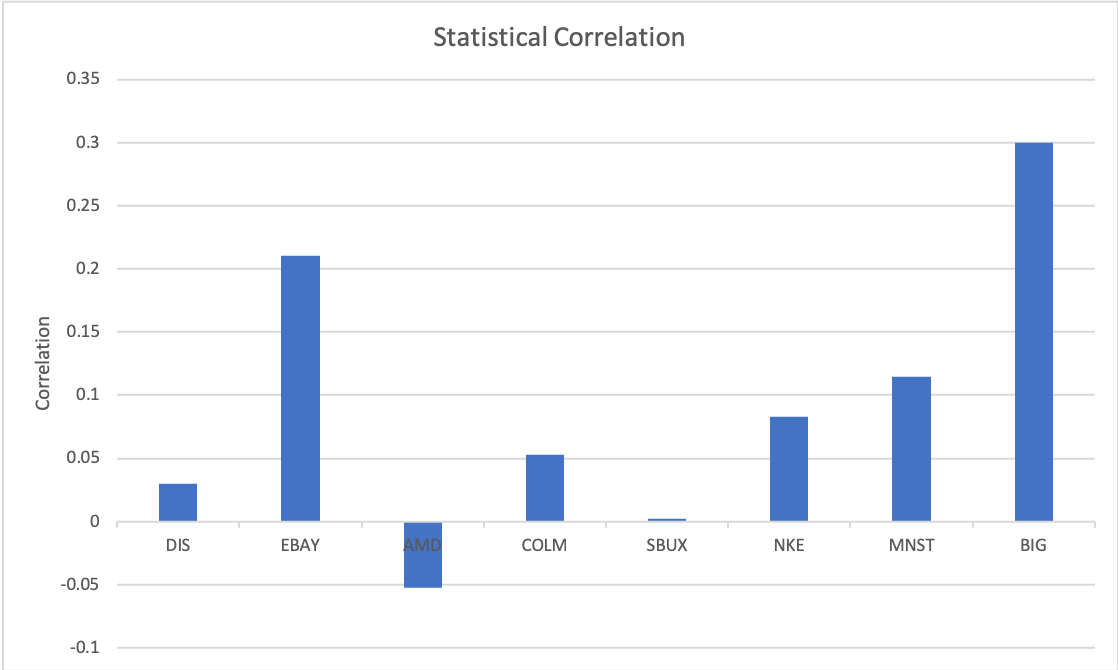
\includegraphics[width=.7\textwidth]{CorrelationResults.png}
\caption{Correlation Results \label{overflow}}
\label{Corrfigure}
\end{figure}

Because there is little correlation between closing price and average sentiment we should expect a na\"{i}ve strategy to perform poorly. We create a simple strategy that generates a buy signal when the average tweet sentiment is above 0.25 and generates a sell signal when it is negative. We rarely find companies that generate overtly negative Twitter content. Most tweets from major companies are often positive, which is logical given the way social media is used for promotion. Therefore, we choose a buy and sell signal threshold that reflects the nature of our dataset. We should expect that if the companies tweets for the day were on average negative, the stock could perform poorly the next day. 

Figure~\ref{Naivefigure} shows the abysmal performance of this na\"{i}ve strategy. Only 25\% of the stocks end up beating the baseline, with the underperforming stocks performing terribly. \texttt{EBAY} characterizes the overall performance of this strategy well -- with the strategy returning 47.2\% while the baseline nets a 237.6\% profit. If sentiment was more correlated with closing price, we would expect this strategy to be more profitable. This lack of correlation motivates the need for a more sophisticated approach, such as using machine learning. 

\begin{figure}[h]
\centering
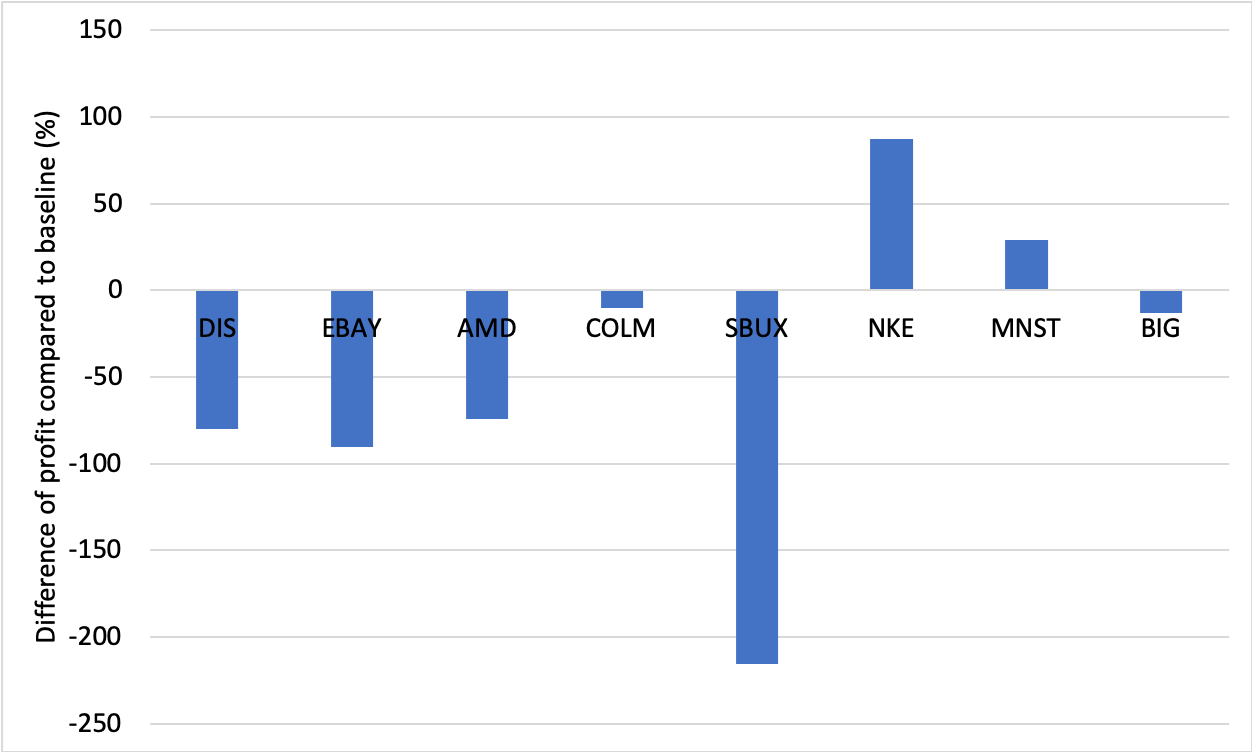
\includegraphics[width=.65\textwidth]{NaiveResults.png}
\caption{Naive Strategy Results \label{overflow}}
\label{Naivefigure}
\end{figure}


\section{Stock Trading and Machine Learning Algorithms}
\label{tradingmlsection}

Our implementation uses the both the \texttt{Scikit-learn} and \texttt{TensorFlow} Python libraries \cite{PedregosaFABIANPEDREGOSA2011} \cite{Abadi}. We use NLP to conduct a sentiment analysis of tweets for our models. We then aggregate the twitter data across days of stock trading and then feed the combined stock and twitter data into different types of machine learning algorithms including trees, $k$-nearest neighbors, and neural networks. We use this variety of machine learning algorithms to attempt to understand if one in particular works well with Twitter sentiment data or if the effectiveness of each algorithm varies from stock to stock. A majority of these models have been used for trading algorithms relying on sentiment in previous literature and have been proven to be effective, further motivating their inclusion in our study \cite{Bollen} \cite{Mao2013} \cite{Shah2014}. We discuss the different types of features inputted to these algorithms in section ~\ref{features}. 

\subsection{Trees}

\subsubsection{Decision Tree Classifier}
Decision trees predict the value of a target variable by learning simple decision rules inferred from the data features \cite{PedregosaFABIANPEDREGOSA2011}. It breaks down a dataset into smaller and smaller subsets, with the leaf nodes representing the classification prediction based on information gain. For features into the classifier, we use the default features specified in the \texttt{Scikit-learn} library. Specifically these features contain: a Gini impurity for criterion, utilizing best split, and using two as the minimum number of samples to split a node. Because we are using a classifier, our implementation predicts whether or not the following days closing price will be higher or lower, which is represented by a 1 or -1. Another benefit of decision trees is that they can be visualized easily. Figure~\ref{DecTreefigure} shows the decision tree fitted to \texttt{DIS}. However, due to the complexity of our model it is difficult to interpret the visualization. 

\begin{figure}[h]
\centering
\includegraphics[width=.6\textwidth]{decision_tree_DIS.pdf}
\caption{Decision Tree Visualization of \texttt{DIS} \label{overflow}}
\label{DecTreefigure}
\end{figure}

\subsubsection{RandomForest Regressor}
Random forests build off of decision trees. It uses a randomized decision tree making a diverse set of classifiers by introducing randomness in the classifier construction \cite{PedregosaFABIANPEDREGOSA2011}. This prediction of the ensemble is then given as an averaged prediction of the individual classifiers. Each tree in the ensemble when it is constructed is built from a random sample drawn from the training set. More randomness is added during construction by choosing the best split of nodes from a random subset of the features. This generally induces more bias from the randomness, but due to averaging often decreases variance and hence yields a better overall model \cite{PedregosaFABIANPEDREGOSA2011}. Just like the features used in the decision tree, we use the default values in the \texttt{Scikit-learn} library. We use 10 trees in the forest and measure quality of a split using mean squared error. Unlike a classifier, a regressor is able to predict and model float values, giving us a different insight, as our implementation predicts the magnitude of change in closing price rather than just the direction of price movement. 

\subsection{$K$-nearest Neighbors Classifier}

This algorithm is one of the simplest machine learning algorithms that exists. After choosing a $k$, or amount of nearest neighbors, it calculates the distance between the query sample and all of the training samples via Euclidian distance \cite{PedregosaFABIANPEDREGOSA2011}. The algorithm then sorts the ordered collection of distances and chooses the mode of the $k$ selected labels for classification. In a regression, it would choose the mean of the $k$ selected labels. For our  algorithm, we choose the default \texttt{Scikit-learn} amount of neighbors: $k=5$. This is motivated by the variety of different features that are used to test the model, generating different groups of neighbors. Future study could take a closer look at this algorithm and identify the ideal amount of neighbors for each particular stock by comparing trading profit across different $k$ values. Because we are doing classification, our algorithm predicts binary price change, as with the other classification algorithms discussed. 

\subsection{Neural Networks}

\subsubsection{MLP Classifier}
An MLP is a neural network that perform binary classification. It has an input layer, a certain number of hidden layers, and an output layer which makes a decision about the given input and are generally used in a supervised learning context. The network \textit{learns} by using a back-propagation algorithm consisting of two steps \cite{Honkela2001}. In the forward pass, predicted outputs from a given input are evaluated mathematically. In the backwards pass, partial derivatives of the cost function are propagated back through the network. Figure~\ref{MLPgraph} shows how a signal flows through a simple MLP with one hidden layer. 

\begin{figure}[h]
\centering
\includegraphics[width=.5\textwidth]{MLP_graph.png}
\caption{Signal-flow graph of an MLP \label{overflow}}
\label{MLPgraph}
\end{figure}

We choose a classifier with 3 hidden layers, each with 100 neurons, and use a stochastic gradient descent for the solver. While MLP classifiers can handle a variety of different layers and solvers, this combination proved to be most effective during testing of the algorithm for our combined Twitter and stock data. The MLP classifier predicts a one or negative one, signaling a price rise or alternatively a price drop the following day. 


\subsubsection{Recurrent Neural Networks - Long Short Term Memory Model}
We implement a deep learning model as well. We utilize a Long Short Term Memory model (LSTM), which is an example of a recurrent neural network (RNN). Unlike traditional neural networks, RNNs use previous data to help classify or predict the current value \cite{Colah2015}. LSTM networks are a special type of RNN that is capable of learning long-term dependencies unliked traditional neural networks which struggle with this problem. They are trained via back-propogation over time and instead of neurons have memory blocks that are connected through layers. Each block contains 3 different types of gates which are triggered by sigmoid activation units: forget, input, and output gates. The first decides wether or not to throw away information from the block. The second decides which values from the input should be allocated to update the memory state. The third decides what to output based on input and memory state. Figure~\ref{lstmfig} demonstrates the architecture of an LSTM model. Because the structure of an RNN allows the model to use past events to aid future states unlike a typical neural network, this has an ideal application for long term time-series based data \cite{Colah2015}. This LSTM model is ideal for our use case, as we utilize time-series stock data. 

\begin{figure}[h]
\centering
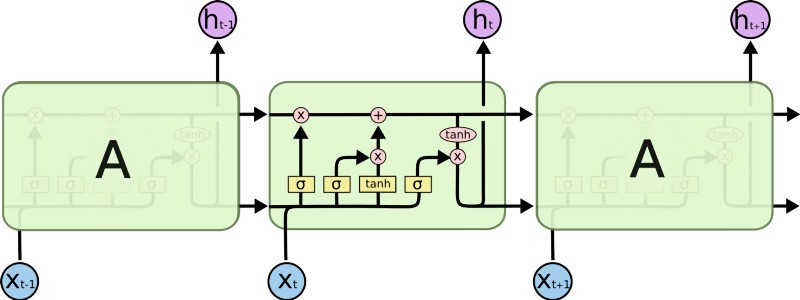
\includegraphics[width=.8\textwidth]{lstmimage.jpeg}
\caption{Architecture of an LSTM model \label{overflow}}
\label{lstmfig}
\end{figure}

The model for our implementation uses a look back of 60 days to give the model enough input to predict the following closing price. At its core, our LSTM model processes 60 days prior of inputs including closing price, tweet sentiment, and a variety of Twitter data, and then predicts the following days closing price. Furthermore, we add a second layer into our model. This stacked LSTM makes the output of the first layer become the input to the second layer, giving our model more depth and accuracy. Unlike the above methods which predict signaled change, this model predicts the stock price.

\subsection{Stacking}
We use stacking to attempt to find more consistent performance with our machine learning algorithms. Stacking works by aggregating the buy and sell signals from each machine learning technique on each day of stock trading. This method is analogous to taking a popular vote, as we trade based on what the majority of the models dictate. We employ two different strategies -- one that behaves more conservatively and another that generates buy signals far more leniently. The former sells all positions if any machine learning model generates a sell signal and only buys when all four models generate a buy signal. The latter gives a buy signal if more than half of the models generate a buy signal and sells if under half give buy signals. By employing these two different strategies, we expect to see more regular performance. 

\section{Feature Sets and Trading Strategy }
\label{features}

We implement a simple trading strategy used across all machine learning techniques. We want to understand the efficacy of particular machine learning techniques, or if a particular model is more effective than the others. For each model, we scale our Twitter data using \texttt{Scikit-learn's} \texttt{minmaxscaler()} preprocessing tool to remove skew, as we find that the majority of companies produce tweets that have far more positive than negative sentiment. 

\subsection{Trading Strategy}

For all of our different machine learning algorithms and models, we use the same simple trading strategy. We buy and sell based on the predicted change in price. Starting with \$1000 of capital, we will buy as many shares as possible if our algorithm predicts that the price will rise the following day. If our algorithm of interest predicts that the price will fall on the following day, we sell all of our positions. We compare against a baseline \textit{buy-and-hold} measure. The baseline is obtained by buying up to \$1000 worth of shares at the beginning of the trading period and selling on the last day. We use two different feature sets for our models, simplistic and complex, and test both using this strategy. 

\subsection{Simplistic Features}

The most simplistic model employed in our research only uses two inputs: closing price and average tweet sentiment.

\subsection{Complex Features}

Building on the simplistic features, we add other twitter features to the input. We use amount of tweets, favorites, and retweets to provide more detailed input to the model, which should translate to more accurate results. We also considered adding more features such as stock volume or moving averages, but we determine that it had no impact on the model. 

\end{document}
